\section{Mesh-Netze}
\label{sec:Mesh-Netzt}

Bei einem Mesh-Netz (vermaschten Netz) handelt es sich um eine Netzwerktopologie. Das Netzwerk kann entweder aus drahtgebunden oder drahtlosen Netzwerkgeräten bestehen. In weiteren Verlauf werden nur drahtlose Netzwerkgeräte betrachtet. Bei einem Mesh-Netz können alle Netzwerkknoten genutzt werden um Daten von Punkt A zu Punkt B zu übertragen. 
\begin{figure}
	\centering
	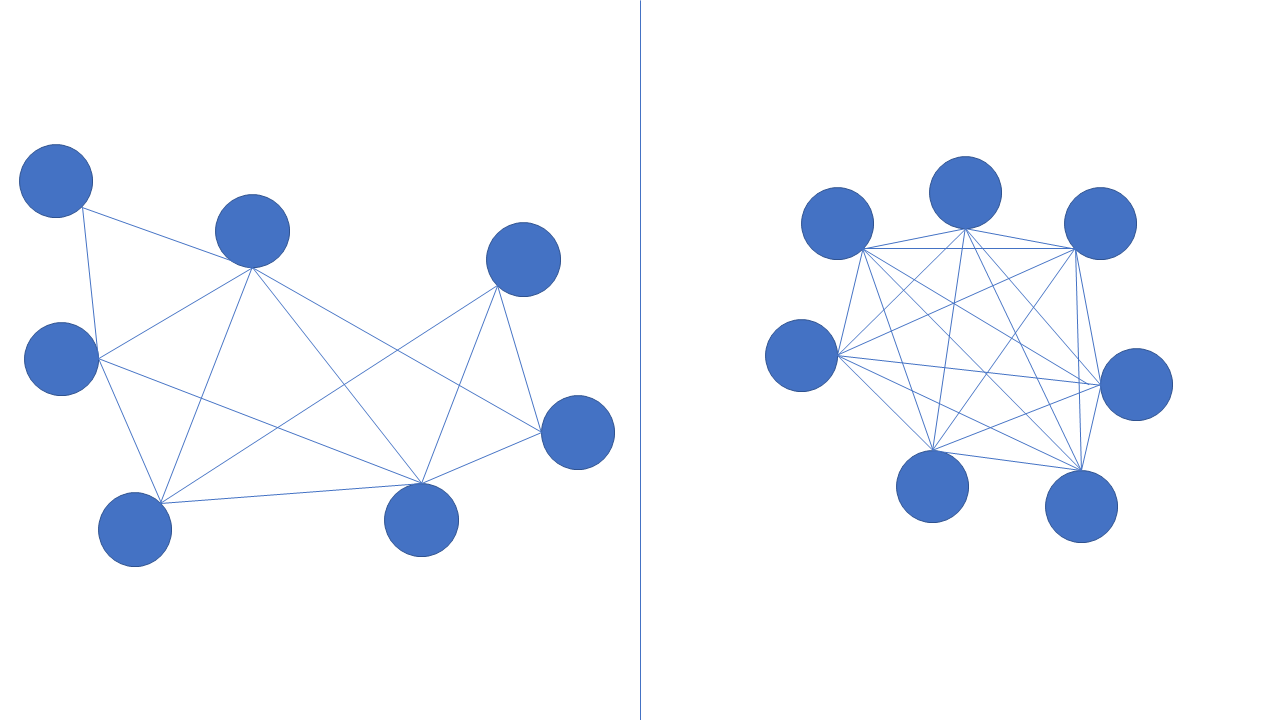
\includegraphics[width=0.9\textwidth]{bilder/vermaschtesNetz.png}
	\caption{Mesh Netzwerk Topologie}
	\label{img:vermaschtesNetz}
\end{figure}

Von einem Mesh Netz wird gesprochen wenn jedes Netzwerkgerät mit mindestens einem oder mehreren Netzwerkgeräten verbunden ist(siehe linke Hälfte der Grafik \ref{img:vermaschtesNetz}). In der Literatur (vgl. \cite{ conrads2013datenkommunikation}) wird in der Regel erst von einem Mesh Netz gesprochen, wenn das Netzwerkgerät über zwei unabhängige Pfade erreicht werden kann, sowie  wenn jedes Netzwerkgerät mit jedem Netzwerkgerät verbunden ist.  Erst dann wird von einem vollständig vermaschten Netz gesprochen (siehe rechte Hälfte der Grafik \ref{img:vermaschtesNetz}). Ein Beispiel für ein teilweise vermaschtes Netzt ist das Internet. 
Bei einem Ausfall eines Knotens/Netzwerkgerät im Mesh Netz können die Daten der anderen Netzwerkgeräte trotzdem an ihr Ziel gelangen. Deshalb ist das Netzt vor allem hinsichtlich seiner Ausfallwahrscheinlichkeit, im Gegensatz zu anderen Netzwerktopologien (zum Beispiel Stern-Topologie), deutlich erhöht. 
Ein Mesh Netz bietet die typischen Netzwerkaufgaben:
\begin{itemize}
	\item Wegsuche (Routing)
	\item Überlastkontrolle (Congestion Control)
	\item Flußkontrolle (Flow Control)
\end{itemize}
Es kann innerhalb eines Mesh Netzwerk zwischen zwei Arten von Netzwerkgeräten unterschieden werden, dem Mesh Router und dem Mesh Clients. Der Mesh Router ist für das gesamte Routing zuständig. Da diese Mesh Router deutlich mehr Funktionen besitzen und deshalb eine höhere Anforderung an die Leistung der Geräte haben, sind diese meist an stationären Punkten aufgestellt. Mesh Clients können jegliche Arten von Geräten sein. Diese Geräte benötigen deutlich weniger Rechenleistungen und müssen deshalb nicht stationär angebracht sein.


Das Routing innerhalb eines Mesh Netzwerk ist eine besondere Herausforderung und kann mit speziellen Mesh Protokolle gemeistert werden. Diese Protokolle lassen sich in drei Kategorien unterteilt werden. Das sind proaktiv, reaktive und hybride Routing Protokolle \cite{vijayakumar2012review}. Bei einem proaktiven Routing Protokoll werden alle Pfade zu allen Knoten, egal ob der Router Daten an diese Knoten senden muss oder nicht, bestimmt. Hierfür wird in periodischen Zeitabständen überprüft ob der Pfad zu den einzelnen Knoten noch verfügbar ist und gegebenenfalls ein neuer Pfad bestimmt wird. Der große Vorteil bei einem proaktiven Vorgehen ist, dass Informationen zum Pfad sehr schnell bereitstehen und diese zur Datenkommunikation verwendet werden können. Bei reaktiven Routing hingegen werden die Pfade nur bestimmt wenn ein Knoten Daten an einen anderen senden möchte. Das Finden des Pfades endet wenn ein Pfad gefunden wurde oder nachdem alle möglichen Kombinationen probiert wurden. Reaktive Protokolle skalieren besser in großen Mesh Netzen. Bei hybriden Routing Protokolle werden beide Ansätze kombiniert.

Trotz einem komplizierten Routing bieten ein drahtloses Mesh Netzt dennoch einige Vorteile gegenüber einem normalen drahtlosen Netz \cite{vijayakumar2012review}:
\begin{itemize}
	\item einfache Breitstellung
	\item hohe Zuverlässigkeit
	\item Selbstkonfiguration
	\item Selbstheilung bei einem Ausfall von Knoten
	\item Skalierbarkeit
\end{itemize}
